\chapter{Introduction}
From 2D, to 3D and now to \acs{bim}. The evolution of the \ac{aec} industry has been a long and complex one. The introduction of 3D modeling was the first major step in the industry's evolution, as it allowed for more accurate representations of buildings. No longer solely relying on 2D drawings, a 3D model of a building can be used to create various representations, from a simple 2D floor plan to a full 3D model. Following the adoption of 3D modeling, the implementation of \ac{bim} emerged as another significant milestone. \ac{bim} adds an extra layer of information on top of the 3D model. As the digital representation of a building's physical and functional characteristics, BIM serves as a repository for semantics originating from various applications throughout the design and construction processes, including cost estimation, energy analysis, and production planning.

\label{sec:intro}
However, as mentioned in \cite{Werbrouck2018}, the next challenge for the \ac{aec} industry is related to the domain-specific nature of current \ac{bim} softwares, which remains closed off to other disciplines. This data management challenge is currently being adressed by the \ac{lbd-cg} and other research entities, such as the University of Ghent, through the use of Web of Data technologies \footcite{ldbimGroup}. This emerging milestone will be discussed in this thesis under the term \ac{ldbim}.

\section{Proposal}
Each of these evolutions has brought, and will continue to bring, a significant amount of data together. This volume is expected to grow exponentially in the future as the industry shifts towards a more digital approach and opens up to other stakeholders. The data graphs will not only expand in terms of semantics but also in geometry. This makes visual querying, or simply put, 3D exploration of models, an increasingly difficult task. Especially when looking at newer devices used in the industry such as mobile phones, and tablets, which are becoming more and more powerful, but still have limited computational resources in comparison to office computers.

To bring this volume of geometric data in perspective, Table \ref{tab:sizeModels} shows the size of the test-models used in \cite{Johansson2015} , a study from 2015 on the performance of \ac{bim} viewers for large models with the following description:

\enquote{
	Although the Hotel model contains some structural elements they are primarily architectural models. As such, no Mechanical, Electrical or Plumbing (MEP) data is present. However, all models except the Hospital contain furniture and other interior equipment.
} \parencite{Johansson2015}

\begin{table}[h]
	\centering
	\begin{tabular}{@{}lrrr@{}}
		\toprule
		Model         & \multicolumn{1}{l}{\# of  triangles} & \multicolumn{1}{l}{\# of objects} & \multicolumn{1}{l}{\# of geometry batches} \\ \midrule
		Library       & 3 685 748                            & 7318                              & 11 195                                     \\
		Student House & 11 737 251                           & 17 674                            & 33 455                                     \\
		Hospital      & 2 344 968                            & 18627                             & 22 265                                     \\
		Hotel         & 7 200 901                            & 41 893                            & 62 624                                     \\ \bottomrule
	\end{tabular}
	\caption{Size of test-models in \cite{Johansson2015}}
	\label{tab:sizeModels}
\end{table}

These models demonstrate how basic \ac{bim} models can already contain a significant amount of data. \ac{ldbim} will not only bring together new stakeholders but also be able to keep track of multiple geometry versions for each object, should they occur. Therefore, this thesis proposes a new approach to the visual querying of \ac{ldbim} models, wherein viewers will not have to load the entire model into memory. Instead, after filtering at the source, only the geometry needed for the visual tasks at hand will be loaded, while maintaining the original link to each resource for further processing and use cases. This filtering step is commonly referred to as culling in the computer graphics industry and is illustrated in Figures \ref{fig:firstIdea} and \ref{fig:cullingPrinciple}.

\begin{figure}[h]
	\centering
	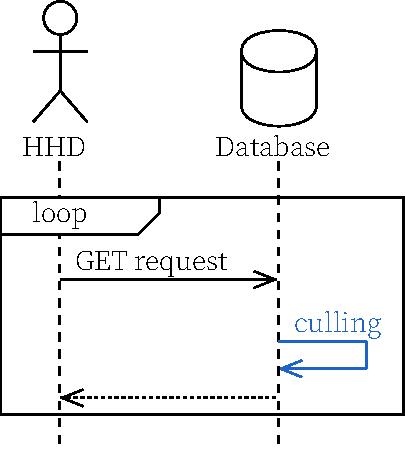
\includegraphics[width=0.4\textwidth]{figures/pdf/first idea.pdf}
	\caption{Sequence diagram - basic concept}
	\label{fig:firstIdea}
\end{figure}

Figure \ref{fig:firstIdea} illustrates the basic idea of this thesis, presenting an extra step in the communication between a user, represented here by a \ac{hhd}, and a database storing the model. An \ac{hhd} has been chosen to exemplify a low-powered device used in the field, which requires a lightweight 3D viewer to visualize and explore the digital twin of the building. The \ac{hhd} is assumed to have no knowledge of the \ac{ldbim} model and only receives the geometry that needs to be displayed from the database. On the other hand, the database is assumed to possess, or have access to, all the knowledge of the model and the necessary semantics to perform the culling. \textcolor{red}{In addition to the culling, Web of Data technologies behind \ac{ldbim} allow for a more flexible approach to data management. The expressive capabilities of \ac{sparql} enable complex and fine-grained queries, in contrast to current \ac{bim} approaches, for data retrieval. This offers a broad range of end-use cases tailored to multiple stakeholders. In this thesis, this translates to user or application-specific query adaptation capabilities.}

\begin{figure}[h]
	\centering
	

% Gradient Info

\tikzset {_lnfkxmyfs/.code = {\pgfsetadditionalshadetransform{ \pgftransformshift{\pgfpoint{0 bp } { 0 bp }  }  \pgftransformrotate{0 }  \pgftransformscale{2 }  }}}
\pgfdeclarehorizontalshading{_mlgazkjgj}{150bp}{rgb(0bp)=(0,0,0);
    rgb(53.839285714285715bp)=(0,0,0);
    rgb(62.5bp)=(0,0,0);
    rgb(100bp)=(0,0,0)}
\tikzset{_ss8aeyqug/.code = {\pgfsetadditionalshadetransform{\pgftransformshift{\pgfpoint{0 bp } { 0 bp }  }  \pgftransformrotate{0 }  \pgftransformscale{2 } }}}
\pgfdeclarehorizontalshading{_jjajrhv3n} {150bp} {color(0bp)=(transparent!90);
    color(53.839285714285715bp)=(transparent!90);
    color(62.5bp)=(transparent!100);
    color(100bp)=(transparent!100) }
\pgfdeclarefading{_vtdml7b05}{\tikz \fill[shading=_jjajrhv3n,_ss8aeyqug] (0,0) rectangle (50bp,50bp); }
\tikzset{every picture/.style={line width=0.75pt}} %set default line width to 0.75pt        

\begin{tikzpicture}[x=0.75pt,y=0.75pt,yscale=-1,xscale=1]
    %uncomment if require: \path (0,300); %set diagram left start at 0, and has height of 300

    %Shape: Polygon [id:ds5156023997500794] 
    \draw  [draw opacity=0][shading=_mlgazkjgj,_lnfkxmyfs,path fading= _vtdml7b05 ,fading transform={xshift=2}] (290.57,117.14) -- (527,29.25) -- (527,281.75) -- (338.71,204.71) -- (331,178.71) -- (339.89,174.11) -- (323.57,171.29) -- (272.43,137.57) -- cycle ;
    %Straight Lines [id:da006883718873094358] 
    \draw    (434,34.25) -- (194,145.75) -- (434,270.25) ;
    %Shape: Polygon [id:ds10437740893464098] 
    \draw  [dash pattern={on 0.84pt off 2.51pt}] (257.86,71.86) -- (275.57,95.57) -- (253,102.43) -- (240.14,86.43) -- cycle ;
    %Shape: Polygon [id:ds4194630640036334] 
    \draw  [dash pattern={on 0.84pt off 2.51pt}] (255,196.43) -- (278.14,219.57) -- (251,229.29) -- (235.57,209.86) -- cycle ;
    %Shape: Polygon [id:ds9339175275440643] 
    \draw  [dash pattern={on 0.84pt off 2.51pt}] (304.14,214.14) -- (321.86,237.86) -- (305,253.86) -- (284.14,239) -- cycle ;
    %Shape: Polygon [id:ds19869780567650053] 
    \draw  [dash pattern={on 4.5pt off 4.5pt}] (471.57,99.57) -- (506.14,123.29) -- (485,155.57) -- (463.57,131) -- cycle ;
    %Shape: Polygon [id:ds9925408688396453] 
    \draw  [dash pattern={on 4.5pt off 4.5pt}] (449.29,150.14) -- (474.43,169.57) -- (479,205.57) -- (441.29,181.57) -- cycle ;
    %Shape: Polygon [id:ds9546564031337637] 
    \draw  [dash pattern={on 4.5pt off 4.5pt}] (402.71,148.43) -- (425.29,169.86) -- (416.14,204.43) -- (394.71,179.86) -- cycle ;
    %Straight Lines [id:da6157949639024258] 
    \draw [color=ugentblue  ,draw opacity=1 ]   (290.57,117.14) -- (272.43,137.57) -- (323.57,171.29) ;
    %Straight Lines [id:da6491410030990774] 
    \draw  [dash pattern={on 4.5pt off 4.5pt}]  (290.57,117.14) -- (357.29,157.29) -- (323.57,171.29) ;
    %Straight Lines [id:da3541991506564892] 
    \draw [color=ugentblue  ,draw opacity=1 ]   (358.29,164.57) -- (331,178.71) -- (338.71,204.71) ;
    %Straight Lines [id:da9181185575223623] 
    \draw  [dash pattern={on 4.5pt off 4.5pt}]  (358.29,164.57) -- (359.57,199.86) -- (338.71,204.71) ;
    %Straight Lines [id:da3449611177421401] 
    \draw    (180.86,129.43) -- (152.43,147.86) -- (183.29,161.57) ;
    %Shape: Ellipse [id:dp5503978735644004] 
    \draw   (168.14,145.71) .. controls (168.14,139.17) and (171.36,133.86) .. (175.32,133.86) .. controls (179.29,133.86) and (182.5,139.17) .. (182.5,145.71) .. controls (182.5,152.26) and (179.29,157.57) .. (175.32,157.57) .. controls (171.36,157.57) and (168.14,152.26) .. (168.14,145.71) -- cycle ;
    %Shape: Ellipse [id:dp8418772956912959] 
    \draw  [draw opacity=0][fill={rgb, 255:red, 0; green, 0; blue, 0 }  ,fill opacity=1 ] (177.25,145.71) .. controls (177.25,143.59) and (178.43,141.87) .. (179.88,141.87) .. controls (181.32,141.87) and (182.5,143.59) .. (182.5,145.71) .. controls (182.5,147.84) and (181.32,149.56) .. (179.88,149.56) .. controls (178.43,149.56) and (177.25,147.84) .. (177.25,145.71) -- cycle ;

    % Text Node
    \draw (174.8,45.4) node [anchor=north west][inner sep=0.75pt]   [align=left] {View-frustrum culling};
    % Text Node
    \draw (318.5,112.5) node [anchor=north west][inner sep=0.75pt]   [align=left] {Back-Face Culling};
    % Text Node
    \draw (261.5,162.5) node [anchor=north west][inner sep=0.75pt]  [color=ugentblue  ,opacity=1 ] [align=left] {visible};
    % Text Node
    \draw (393.5,207.5) node [anchor=north west][inner sep=0.75pt]   [align=left] {Occlusion Culling};
    % Text Node
    \draw (345.77,230.25) node [anchor=north west][inner sep=0.75pt]  [font=\footnotesize,rotate=-27.04] [align=left] {View Frustrum};


\end{tikzpicture}

	\caption[Illustration of culling principle]{Illustration of culling principle, based on \cite{CullingPrinciples}}
	\label{fig:cullingPrinciple}
\end{figure}

Figure \ref{fig:cullingPrinciple} showcases multiple culling techniques to showcase some culling principles. The first technique, \emph{frustum culling}, is used to determine which objects are visible to the user. The second technique, \emph{occlusion culling}, is used to determine which objects are occluded by or behind other objects. And lastly, \emph{back-face culling}, is used to determine which faces, and not whole objects, are facing away from the user.

\section{Research questions}\label{sec:researchQuestions}
This thesis proposes the introduction of culling algorithm technology within the context of \ac{ldbim} to address the previously mentioned issue of the scene's size, by culling the scene at its source prior to sending it to the viewer. As culling algorithms have been extensively researched and continue to evolve, as described in section \ref{sec:historyCulling}, the research questions in this thesis concentrate on assessing the feasibility of introducing such algorithms in \ac{ldbim}. It aims to propose a set of possible solutions tailored to this specific problem, while highlighting possibilities for future research and specific use cases.

\subsection[Can \acs{ldbim} be culled?]{To what extent can \acs{ldbim} geometry be culled \\
	to be streamed to lightweight viewers?}

This thesis focuses on computing with data snippets or triples inside a \ac{ldbim} model, rather than within. This means that the smallest unit of data that can be culled is the one described in a single triple, which is, in the most likely scenario, a single \ac{lod} of a single element. It implies that geometry is defined and separated at the object level. Furthermore, this thesis will not address culling techniques such as back-face culling, as these will be left to the viewer itself, not the database.

Determining the necessary data snippets for the viewer is a key question. The fundamental requirements for the viewer include, first, the geometry itself, which involves selecting the appropriate geometry format for the application as well as the additional visual information such as color, texture, etc. Second, the identifier of each element is of crucial importance in order to maintain the link to other semantic resources in the graph. This enables the viewer to retrieve those resources for a multitude of use cases, transforming it into a user-friendly visual query tool.

\subsection[Can existing semantics be used?]{Can existing semantics and ontologies be used\\
	to feed possible culling algorithms?}\label{subsec:rq2}
Unlike the computer graphics industry, this interconnected context already contains both explicit and implicit relationships within the graph, the latter being derived through inferencing. This is similar to \cite{Johansson2009} and their paper where they utilized the semantics of a \ac{bim} model in \ac{ifc} format to develop culling techniques. However, this thesis will concentrate on the use of Semantic Web resources. As such, it will examine both \ac{aec}-specific and \ac{aec}-related ontologies, such as those related to \ac{gis}, to determine if they can be employed to feed culling algorithms.
